%%%%%%%%%%%%%%%%%%%%%%%%%%%%%%%%%%%%%%%%%
% Journal Article
% LaTeX Template
% Version 1.3 (9/9/13)
%
% This template has been downloaded from:
% http://www.LaTeXTemplates.com
%
% Original author:
% Frits Wenneker (http://www.howtotex.com)
%
% License:
% CC BY-NC-SA 3.0 (http://creativecommons.org/licenses/by-nc-sa/3.0/)
%
%%%%%%%%%%%%%%%%%%%%%%%%%%%%%%%%%%%%%%%%%

%----------------------------------------------------------------------------------------
%	PACKAGES AND OTHER DOCUMENT CONFIGURATIONS
%----------------------------------------------------------------------------------------

\documentclass[twocolumn]{article}

%% Load graphicx package
\usepackage{graphicx}
%\usepackage[font=small]{subfig}
\graphicspath{{images/}}
\DeclareGraphicsExtensions{.pdf,.png,.jpg}
%\usepackage{amsmath}
\usepackage[font=small]{subfig}

\usepackage{lipsum} % Package to generate dummy text throughout this template

\usepackage[sc]{mathpazo} % Use the Palatino font
\usepackage[T1]{fontenc} % Use 8-bit encoding that has 256 glyphs
\linespread{1.05} % Line spacing - Palatino needs more space between lines
\usepackage{microtype} % Slightly tweak font spacing for aesthetics

\usepackage[hmarginratio=1:1,top=32mm,columnsep=16pt]{geometry} % Document margins
%\usepackage{multicol} % Used for the two-column layout of the document
\usepackage[hang, small,labelfont=bf,up,textfont=it,up]{caption} % Custom captions under/above floats in tables or figures
\usepackage{booktabs} % Horizontal rules in tables

\usepackage{hyperref} % For hyperlinks in the PDF

\usepackage{paralist} % Used for the compactitem environment which makes bullet points with less space between them

\usepackage{abstract} % Allows abstract customization
\renewcommand{\abstractnamefont}{\normalfont\bfseries} % Set the "Abstract" text to bold
\renewcommand{\abstracttextfont}{\normalfont\small\itshape} % Set the abstract itself to small italic text

\usepackage{titlesec} % Allows customization of titles
\renewcommand\thesection{\Roman{section}} % Roman numerals for the sections
\renewcommand\thesubsection{\Roman{subsection}} % Roman numerals for subsections
\titleformat{\section}[block]{\large\scshape\centering}{\thesection.}{1em}{} % Change the look of the section titles
\titleformat{\subsection}[block]{\large}{\thesubsection.}{1em}{} % Change the look of the section titles

\usepackage{fancyhdr} % Headers and footers
\pagestyle{fancy} % All pages have headers and footers
\fancyhead{} % Blank out the default header
\fancyfoot{} % Blank out the default footer
\fancyhead[C]{European Wind Energy Association Conference  $\bullet$ March 2014 $\bullet$ Barcelona, Spain} % Custom header text
\fancyfoot[RO,LE]{\thepage} % Custom footer text

%----------------------------------------------------------------------------------------
%	TITLE SECTION
%----------------------------------------------------------------------------------------

\title{\vspace{-15mm}\fontsize{24pt}{10pt}\selectfont\textbf{Sizing of Electrical Generators for a Floating OWC Array}} % Article title

\author{
\large
\textsc{Ozan Keysan, Markus A. Mueller}\thanks{Institute of Energy Systems, University of Edinburgh}\\[2mm] % Your name
\normalsize Institute of Energy Systems, University of Edinburgh \\ % Your institution
\normalsize \href{mailto:o.keysan@ed.ac.uk}{o.keysan@ed.ac.uk} % Your email address
\vspace{-5mm}
}
\date{}

%----------------------------------------------------------------------------------------

\begin{document}

\twocolumn[
\begin{@twocolumnfalse}

\maketitle % Insert title

%\thispagestyle{fancy} % All pages have headers and footers


\begin{abstract}

Floating wind and wave energy platforms can help to exploit far offshore renewable energy resources.
However, the cost of these devices are higher than the onshore equivalents. The cost of the power take-off system can be reduced by reducing the generator power rating, which will increase the capacity factor. Annual energy income is estimated with different sized generators using  an oscillating water column model. The parameters used in mechanical and electrical models are presented in the paper as a function of generator's power rating.
\end{abstract}

\end{@twocolumnfalse}
]
%\begin{multicols}{2} % Two-column layout throughout the main article text

\section{Introduction}

Deep water renewable energy resources remained mostly untapped so far due to difficulties in installation. However, offshore wind regimes are more regular and wind speeds are higher. The average offshore wind speed is around 8.6 m/s, almost double of the average onshore wind speed, which is around 4.6~m/s~\cite{Hau2013}. On top of that, there is also large resource of wave energy, which is around 70 kW/m off the West coast of Scotland \cite{BERR2008}. Floating combined wind-wave energy platforms offshore energy platforms can be used to exploit these energy resources.

MARINA Platform is an EU FP7 project that aims to design different combined floating wind and wave energy platforms \cite{marinaweb}. The project evaluated various combined wind and wave energy platforms in terms of manufacturability, cost of energy, reliability etc. \cite{Barrios2012}. Main challenges in offshore floating platforms is the high installation and maintenance costs. The cost of the system can be minimised by reducing the size of the power take-off system.

One of the concepts is a floating platform that consists of a 5~MW wind turbine and 20 oscillating water columns (OWC) as shown in Fig.~\ref{owc_array}). Each OWC has a maximum rating of 500~kW \cite{Sullivan2013}.

  \begin{figure}
    \centering
    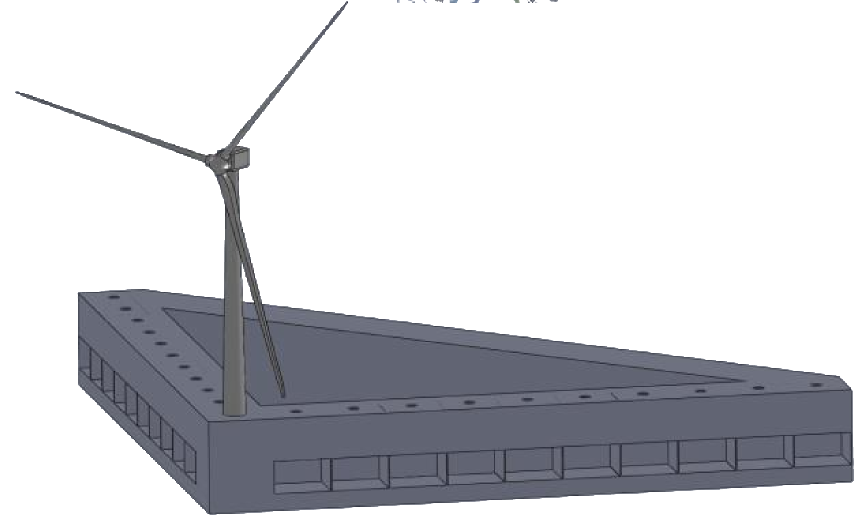
\includegraphics[]{owc_array}
    \caption{Floating OWC array with single wind turbine concept \cite{Sullivan2013}.} 
    \label{owc_array}
  \end{figure}

The power take-off system of the wind turbine consists of a doubly-fed induction generator (DFIG) coupled to a multi-stage gearbox \cite{Jonkman2009}. In the OWC, prime mover is a Well's turbine, a symmetrical turbine which rotates in the same direction regardless of the direction of air flow. In contrast to wind turbines, Well's turbines usually don't have any pitch control mechanism, thus the output power is directly related to the air speed in the OWC chamber. In the OWC concept the Well's turbine is directly coupled to a rotary generator. The generator speed should be adjusted to keep angle of attack in the blades within a small range to maximise the energy extract.

%------------------------------------------------

\section{Generator Type}

Squirrel cage induction generators (SCIG) have simple and robust structure, which makes them suitable for a wave energy converter of a floating OWC platform, where access is limited by weather and sea conditions and any repairs in the OWC chamber are challenging. 
The most suitable SCIG type for floating offshore platforms are special-made marine motors, which are widely used in ships. In particular, motors used on deck have very similar operating conditions with the electrical generators of OWCs. They both operate in humid and saline environment with occasional water sprays and flooding. Also in a floating platform, there is continuous rolling motion and wide range of ambient temperature. Marine induction machines can be manufactured  with cast iron frames to reduce corrosion, can be painted with special paints or can have higher level of insulations (IP56 or IP65).

\begin{table}
  \centering
  \begin{tabular}{cc}
    \hline
Av. Wind Speed & 6.98 m/s \\
Av. Wave Power & 42.7 kW/m \\
Av. Wave Period & 11.84 s \\
Significant wave & 10.2 m  \\
(50-year) \\
\hline
  \end{tabular}
  \caption{Specifications of the selected site (Site~\#3: off the coast of Spain and Portugal)\cite{Gao2012}.}
  \label{site_spec}
\end{table}

\begin{figure}[t]
  \centering
  \subfloat[Significant wave height distribution.]{\label{generator_inertia}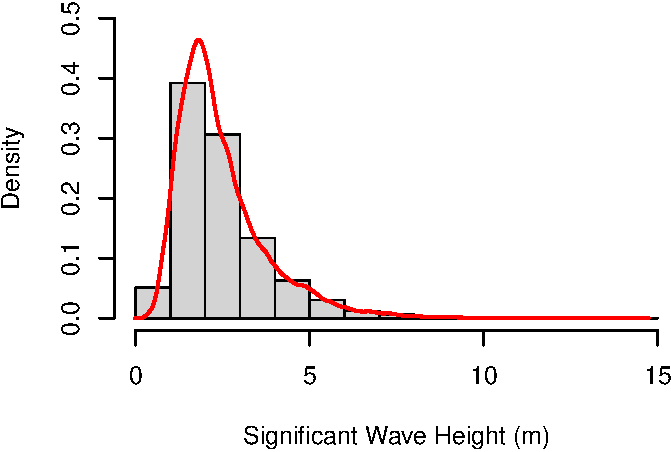
\includegraphics[width=0.45\textwidth]{spain_significant_wave}}

  \subfloat[Mean swell period distribution.]{\label{time_constant}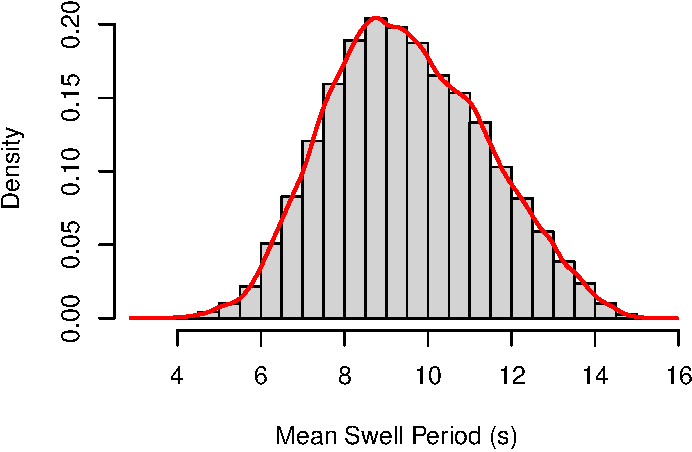
\includegraphics[width=0.45\textwidth]{spain_mean_swell}}
    \caption{Probability distribution for the wave characteristics of site \#3 (between 2001 and 2010).} 
    \label{spain_site}
\end{figure} 

\section{Generator Sizing}

The cost of the power take-off system is directly proportional to the power rating of the generator. Furthermore, the cost of power electronics, circuit breakers etc. are also related to the generator size. The usual practice is to choose the generator rating according to the maximum power rating of the OWC. However, in this case the capacity factor of the generator will be low throughout the year. It will be fully utilised just for a short amount time when there are high seas. However, choosing a smaller generator can reduce the annual energy generation as the power output is now limited by the rating of the generator.

In order to estimate the optimum power rating, resource data supplied by the partners of the MARINA Platform project is used \cite{Gao2012}. Among many possible places, site site \#3, which is off the coast of Portugal and Spain, is chosen because of having both high wind and high wave energy resource. The main specifications of the site are presented in Table~\ref{site_spec}. In Fig.~\ref{spain_site} the significant wave height distribution and mean swell period distribution of the site are given. Typical energy input is presented in Fig.~\ref{power_input}.




  \begin{figure}[]
    \centering
    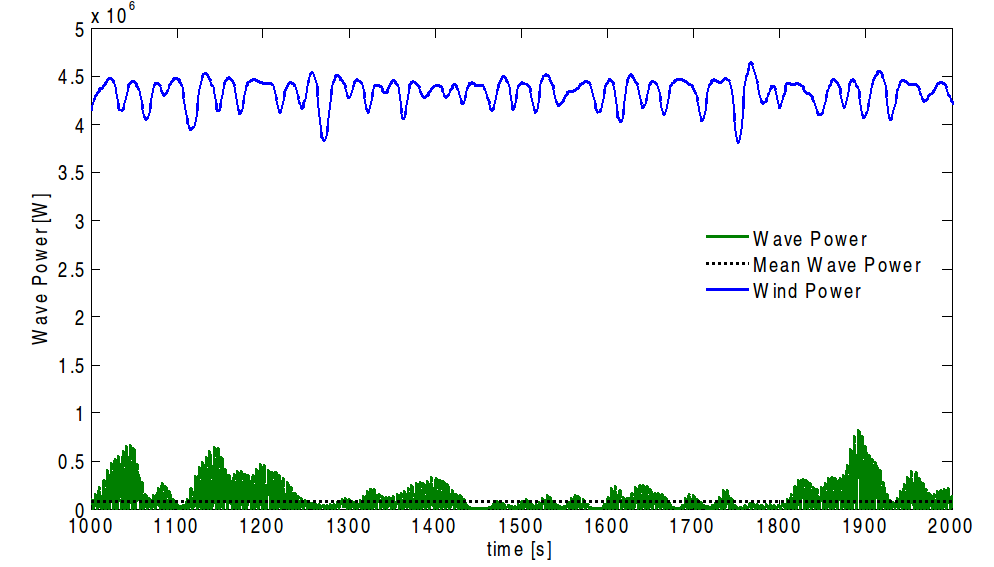
\includegraphics[width=0.5\textwidth]{power_input}
    \caption{Typical power output from the wind turbine and wave energy converter.} 
    \label{power_input}
  \end{figure}

Annual energy generation versus the generator power rating is calculated using the time-series data between 2001 and 2010 and the results are presented in Fig.~\ref{generator_rating} and in Table~\ref{generator_rating_table}. A 500~kW generator produces 670~MWh/year. Reducing the generator rating to 250~kW reduces the energy harvest just by 10~\%. In other words for the extra 70~MWh, the generator capacity has to be doubled, which makes the extra 70~MWh nine times more expensive than the first 600~MWh. It is also possible to get more power from generators due to improved thermal performance as shown in \cite{Hodgins2010a}. In this case, the size of the generator can be further reduced. 

However, it should be noted that, the total cost of the system is dominated by the cost of structure and installation, and the cost of the generator is only a small fraction of it. On the other side, reducing the generator size also cuts down the cost of power electronics, circuit breakers, transformer etc.

  \begin{figure}[]
    \centering
    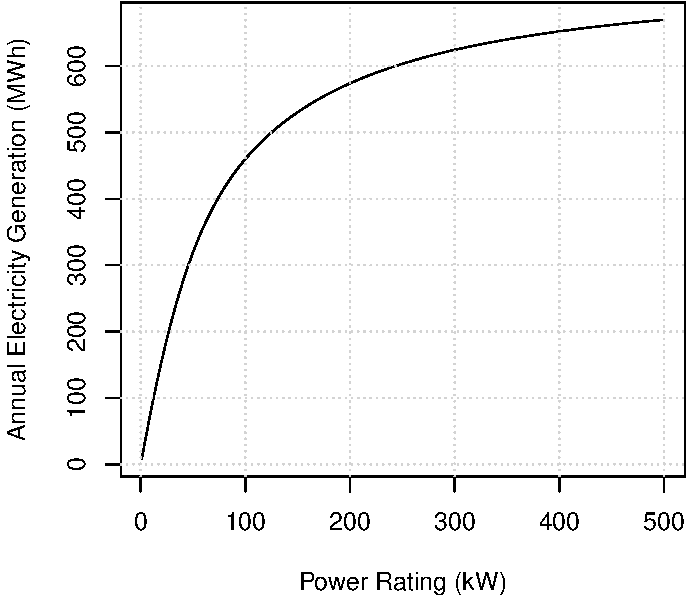
\includegraphics[width=0.5\textwidth]{generator_rating}
    \caption{Annual energy generation from single OWC as a function of the generator rating.} 
    \label{generator_rating}
  \end{figure}
  
  \begin{table}[t]
    \centering
    \begin{tabular}{ccc}
     Generator & Annual & Normalized \\
     Rating & Energy & (\%) \\
    \hline
  200 kW & 574 MWh & 85.7 \% \\
  250 kW & 603 MWh & 90.0 \% \\
  300 kW & 624 MWh & 93.1 \% \\
  400 kW & 652 MWh & 97.3 \% \\
  500 kW & 670 MWh & 100 \%\\
  \hline
    \end{tabular}
    \caption{Annual energy generation variation with generator power rating}
    \label{generator_rating_table}
  \end{table}
  

\section{Generator Parameter Estimation}

In order to evaluate the performance of the combined wind-wave energy systems for different ratings of the generator, a combined Simulink model is developed in the MARINA Platform project. Different power aggregation methods can be applied, which will be presented in a different paper.

An accurate generator model for each power rating is required. In Simulink, electrical generators are modelled using a mechanical and an electrical system. Mechanical system is defined by rotor inertia and friction constant. The electrical system is represented using the equivalent electric circuit presented in Fig. \ref{equivalent_circuit}. In the circuit $R_s, R_r$ are the stator and rotor resistance, $L_{ls}, L_{lr}$ are the stator and rotor leakage inductance, $L_m$ is the magnetising inductance.


  \begin{figure}
    \centering
    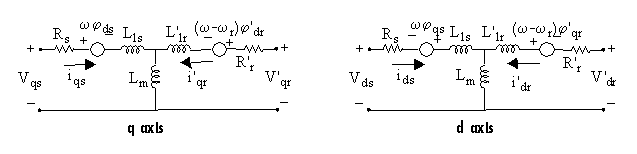
\includegraphics[width=0.5\textwidth]{scig_schematic}
    \caption{Equivalent circuit of an induction machine \cite{matlab2014}.} 
    \label{equivalent_circuit}
  \end{figure}
  
\subsection*{Rotor Inertia}

The rotor inertia($J$), which has a direct effect in the transient response of the machine, is especially important in variable speed systems as in OWC. The inertia depends on the rotor dimensions, which depends on the rated power and number of poles. Inertia of several machines are collected from commercial machine catalogues \cite{Siemens2012} and plotted in Fig.~\ref{generator_inertia}. The trend lines for these data are calculated and the equations are presented in Table~\ref{inertia_estimation}.

It is possible to convert the rotor inertia ($kgm^2$) to mechanical time constant (seconds), which is commonly used in the per unit system.  Time constant is the ratio of rotational kinetic energy stored in the rotor to the power rating of the machine. Inertia values presented in Fig.~\ref{generator_inertia} are converted to time constant using eq. (\ref{eq:time_constant}) and the results are presented in Fig.~\ref{time_constant}. The equation of the trend line is given in eq. (\ref{eq:time_constant_trend}).


\begin{figure}[]
  \centering
  \subfloat[Rotor Inertia.]{\label{generator_inertia}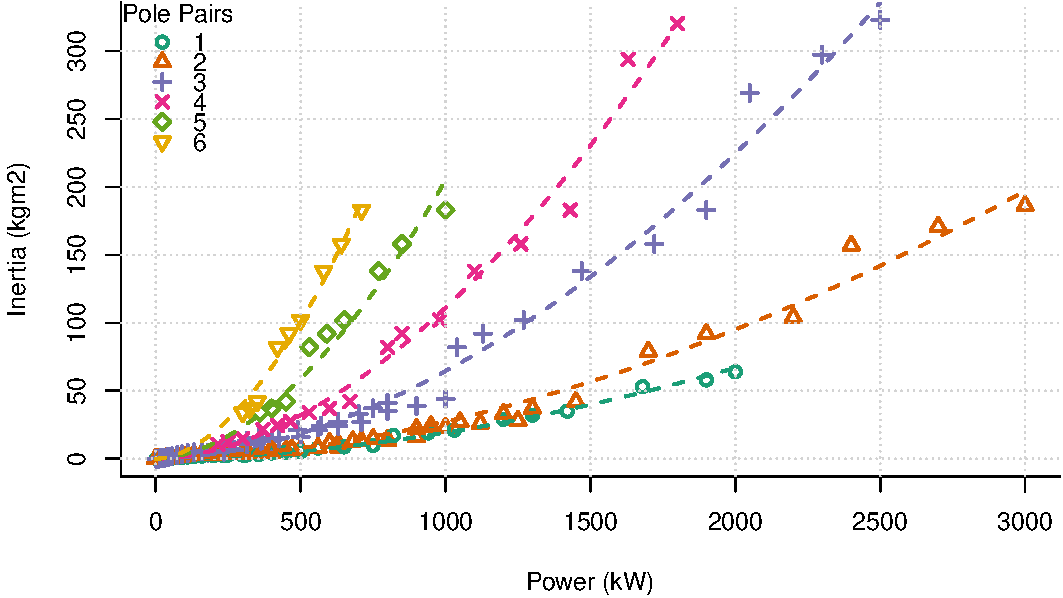
\includegraphics[width=0.5\textwidth]{generator_inertia}}

  \subfloat[Time constant.]{\label{time_constant}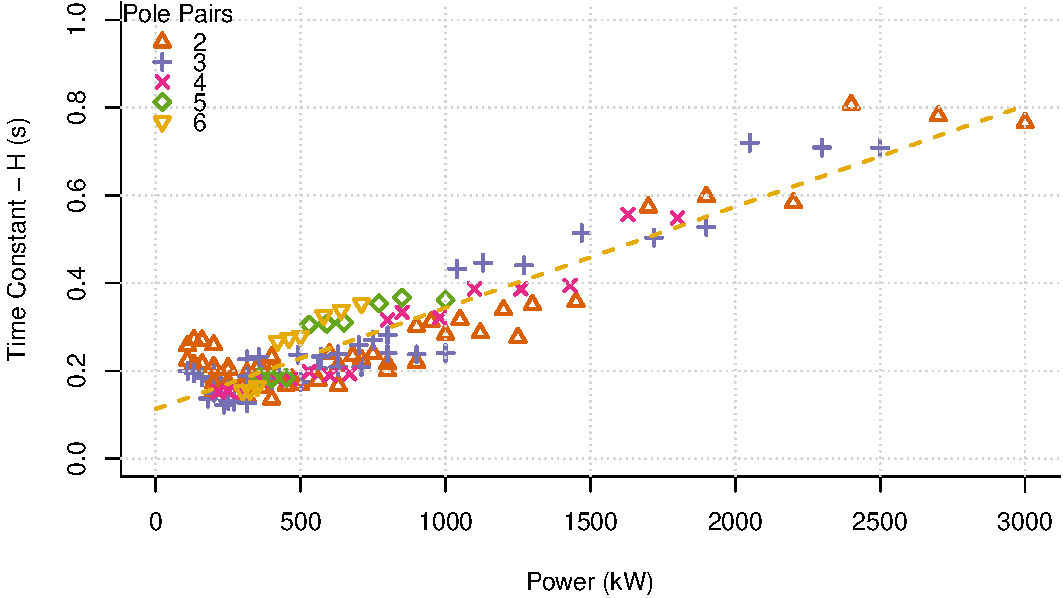
\includegraphics[width=0.5\textwidth]{time_constant}}
    \caption{The rotor inertia and rotor time constant variation as function of pole number and rated power.} 
    \label{inertia_timeconstant}
\end{figure}


\begin{equation}
	H(s)=\frac{\frac{1}{2} J {w_{mech}}^2}{P_{rated}}
	\label{eq:time_constant}
\end{equation}

\begin{equation}
	H(s)=0.00023 \times P_{(kW)} + 0.11335
	\label{eq:time_constant_trend}
\end{equation}

\begin{table*}
  \centering
  \begin{tabular}{lll}
   $N_{pole}$ & Small Machines (<100 kW) & Large Machines (>100 kW) \\
  \hline
2 & $315\times10^{-6}\times {P_{(kW)}}^{1.784}$ & $76\times10^{-6}\times {P_{(kW)}}^{1.8}$ \\
4 & $847\times10^{-6}\times {P_{(kW)}}^{1.68}$ & $109\times10^{-6}\times {P_{(kW)}}^{1.8}$ \\
6 & $4367\times10^{-6}\times {P_{(kW)}}^{1.471}$ & $257\times10^{-6}\times {P_{(kW)}}^{1.8}$ \\
8 &  & $442\times10^{-6}\times {P_{(kW)}}^{1.8}$ \\
10 & & $816\times10^{-6}\times {P_{(kW)}}^{1.8}$ \\
12 & & $1393\times10^{-6}\times {P_{(kW)}}^{1.8}$ \\
\hline
  \end{tabular}
  \caption{Rotor Inertia($kg m^2$) estimation for induction machines as a function of number of poles and rated power.}
  \label{inertia_estimation}
\end{table*}


\subsection*{Electrical Parameters} % (fold)
\label{sub:electrical_parameters}

Similar approximations are performed for the electrical parameters of the induction generator using the manufacturer's data and data presented in \cite{Thiringer2001}.
It is easier to represent these parameters in per unit system. The stator resistance variation (in per unit) as a function of the rated power is presented in Fig.~\ref{Rs}. It can be seen from the Fig.~\ref{Rs_log_plot} that the stator resistance changes linearly in the logarithmic scale. The stator resistance can be estimated as:

\begin{equation}
 	ln(R_s(pu))=-0.3772\;ln (P_{(kW)}) - 2.441
 	\label{eq:Rs}
 \end{equation} 

\begin{figure}[]
  \centering
  \subfloat[Linear Y-axis.]{\label{Rs_plot}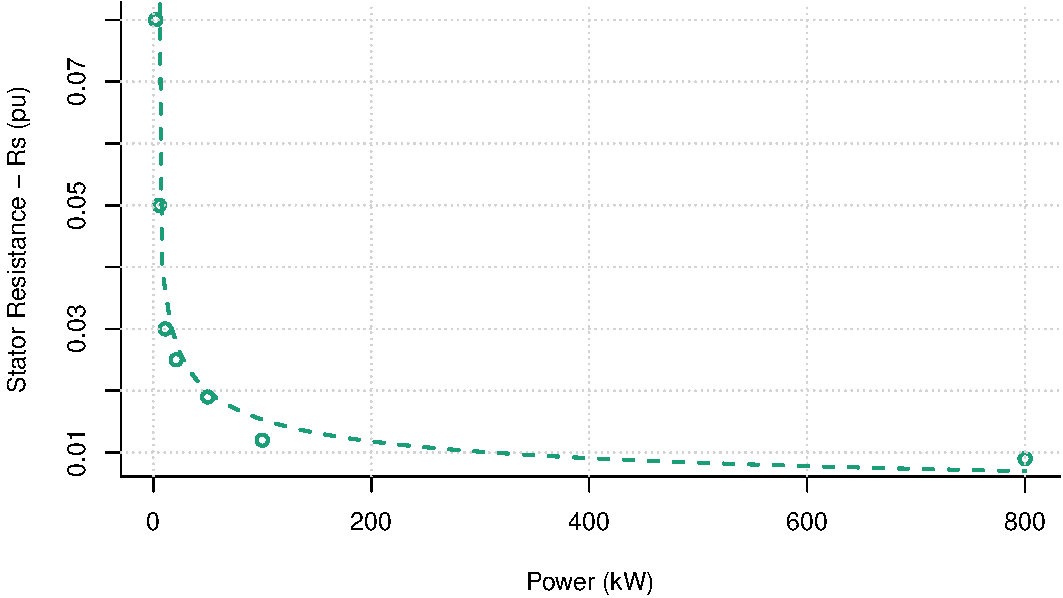
\includegraphics[width=0.5\textwidth]{Rs_plot}}

  \subfloat[Logarithmic Y-axis.]{\label{Rs_log_plot}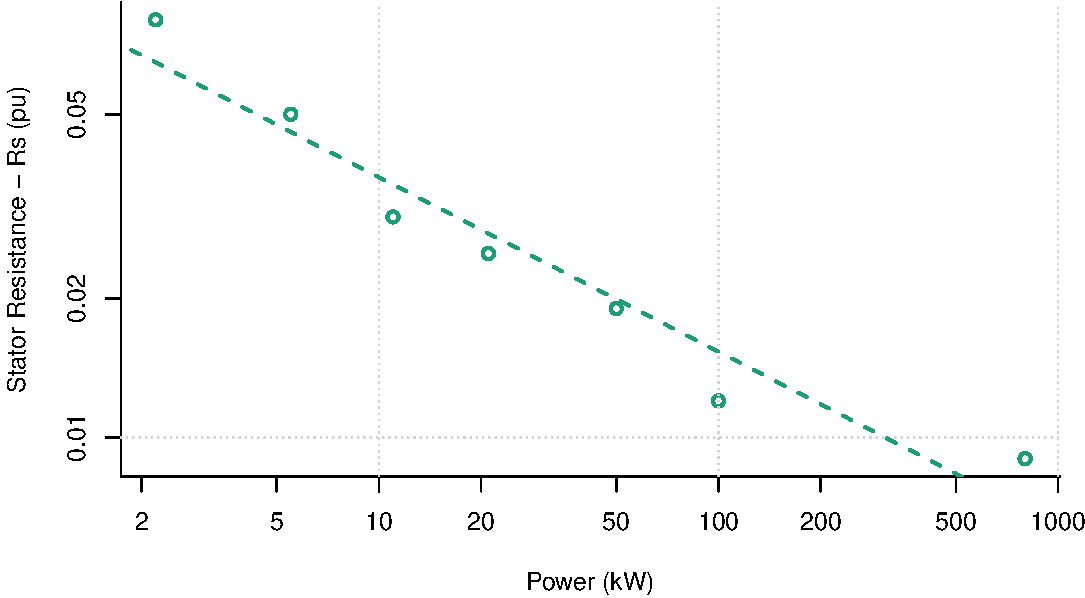
\includegraphics[width=0.5\textwidth]{Rs_log_plot}}
    \caption{Rotor resistance (in per unit) variation as a function of the rated power.} 
    \label{Rs}
\end{figure}

Magnetising inductance ($L_m$) defines the flux linkage between stator and rotor. The magnetising inductance as a function of the power rating is presented in Fig. \ref{Lm_plot}. Another parameter is the leakage inductance, which is related to leakage flux in the machine and has a direct effect on the power factor. The leakage inductance as a function of the rated power is presented in Fig. \ref{Lls_plot}. Magnetising and leakage inductances can be estimated as follows:

\begin{equation}
 	L_m (pu) = 0.158\;ln (P_{(kW)}) + 2.23
 	\label{eq:Lm}
 \end{equation} 

\begin{equation}
 	L_{ls}(pu) = -0.3772 \;ln (P_{(kW)}) - 2.441
 	\label{eq:Lls}
 \end{equation} 


\begin{figure}[]
  \centering
  \subfloat[Mutual inductance, $L_m$.]{\label{Lm_plot}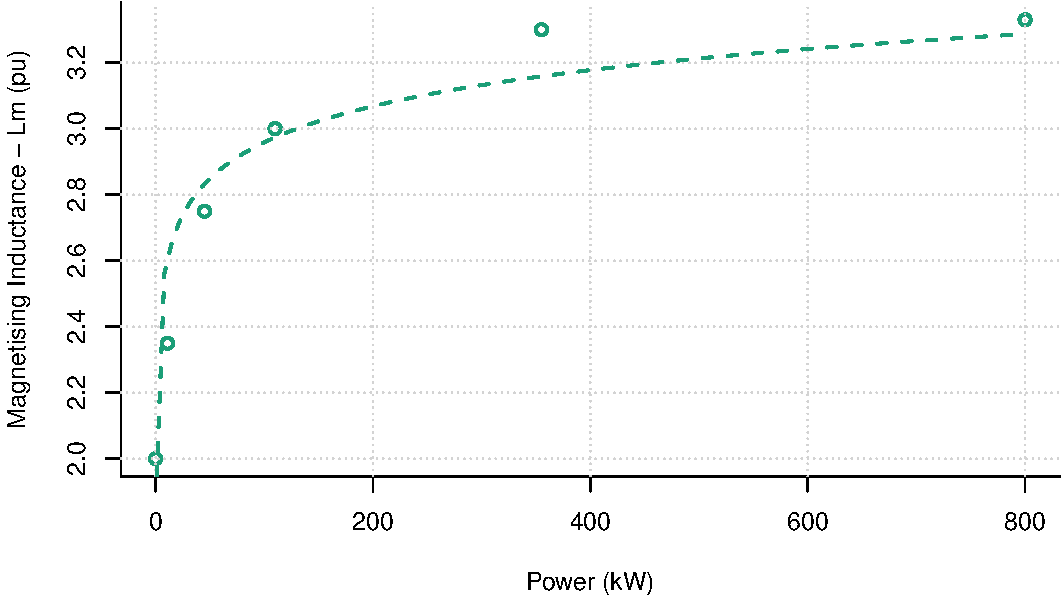
\includegraphics[width=0.5\textwidth]{Lm_plot}}

  \subfloat[Stator leakage inductance, $L_{ls}$.]{\label{Lls_plot}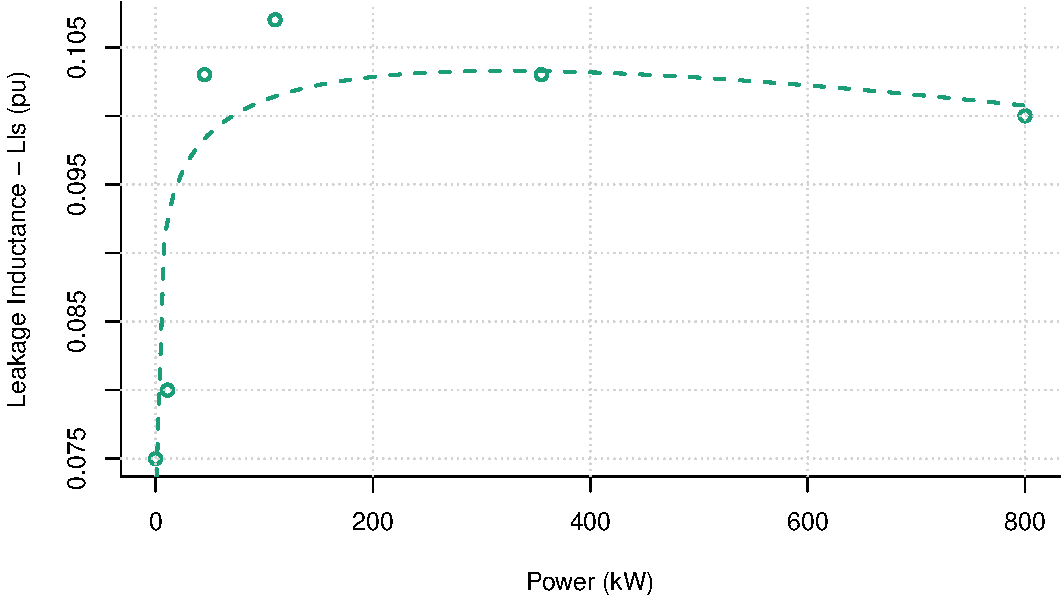
\includegraphics[width=0.5\textwidth]{Lls_plot}}
    \caption{Variation of mutual and stator leakage inductance (in per unit) as a function of the rated power.} 
    \label{inductance_plots}
\end{figure}

% subsection electrical_parameters (end)

\section{Conclusion}

Variation of annual electricity generation with generator rating is estimated for a floating OWC array. It is shown that in the current OWC design single OWC with a 500 kW generator produces 670 MWh per year. Reducing generator rating to 250 kW just reduces the annual energy output by 10~\%. The capacity factor for a 500 kW generator is 0.153 and increases to 0.275 for the 250 kW generator. Although it is not included in this paper, it is shown in \cite{Hodgings2010a} that generators in OWCs can generate more power than onshore equivalents due to improved cooling. In this way, it is possible to further reduce the generator rating.

The electrical and mechanical parameters for the generator models are also presented. It is believed that these equations will help anyone that wants to model various machines analytically. The equations and datasets are made publicly available in XXX. 

\section*{Acknowledgement} % (fold)
\label{sec:acknowledgement}

The authors gratefully acknowledge the financial support
from the EU FP7 MARINA Platform project, grant agreement no. FP7-241402.
% section acknowledgement (end)
%------------------------------------------------

%----------------------------------------------------------------------------------------
%	REFERENCE LIST
%----------------------------------------------------------------------------------------
\bibliography{ewea-2014}

\bibliographystyle{ieeetr}

%----------------------------------------------------------------------------------------

%\end{multicols}

\end{document}
